\chapter{Marco teórico y estado del arte}


Esta tesis busca presentar una nueva alternativa para la caracterización de comunidades microbianas utilizando secuenciación de tercera generación. Para ello se  desarrolló un flujo de trabajo automatizado que permite realizar el procesamiento de los datos de secuenciación, control de calidad, asignación taxonómica, análisis de diversidad, predicción funcional y caracterización de grupos. 
Se desarrolló también una aplicación web que ejecuta el flujo de trabajo y presenta los resultados en forma de gráficos y tablas en la plataforma. Para usar la plataforma el usuario debe llenar un formulario con la metadata de la secuenciación, subir los archivos e indicar los análisis a realizar, con esto la plataforma web enviará los datos de secuenciación a la plataforma de alto rendimiento y ejectará el flujo de trabajo, una vez finalizado, los resultados se presentarán en la plataforma web.

A continación se presenta el marco teórico y estado del arte de los conceptos necesarios para el desarrollo de esta tesis, como qué es la microbiota, el gen 16S rRNA, tecnologías de secuenciación y sus usos, las diferentes herramientas bioinformáticas para el análisis de datos y herramientas para el desarrollo de la aplicación web.
\section{Gen 16S para el estudio de comunidades microbioanas /  Estudio de microbiota a traves del gen 16S y tecnologías de secuenciacion}
\subsection{Microbiota}
La microbiota es el conjunto de microorganismos (bacterias, virus, arqueas, u hongos) que habitan en un ambiente, ya sea en organismos multicelulares como humanos~\cite{gilbert2018current}, animales~\cite{bahrndorff2016microbiome} o plantas~\cite{berendsen2012rhizosphere}, y también en ambientes naturales como el océano~\cite{doi:10.1126/science.aac8455} y el suelo~\cite{banerjee2023soil}. Estos organismos que componen la microbiota se encuentran en un estado de simbiosis junto con el huesped, contribuyendo en funciones vitales como la homeostasis, regulación del sistema inmune, digestión de alimentos, producción de vitaminas, protección ante enfermedades y agentes patógenos~\cite{marco2021defining,fijan2014microorganisms,altvecs2020interaction,hou2022microbiota}. Sin embargo, una disbiosis o una baja diversidad en la microbiota puede llevar a una desregulación en el organismo huesped, incluyendo diversos tipos de enfermedades, fallas en el sistema inmune, falta de vitaminas, trastornos como depresión, estrés, e incluso diferentes tipos de cáncer en el caso del ser humano~\cite{altvecs2020interaction,hou2022microbiota}.

La composición de la microbiota va cambiando dependiendo del área de estudio, pudiéndose encontrar diferentes microorganismos en las cavidades orales, zonas intestinales, genitales, cutáneas o tracto respiratorio~\cite{ursell2012interpersonal}.

Se estima que en el ser humano habitan más de 10 billones de microorganismos~\cite{sender2016revised}, es decir, poseemos cerca de 350 billones de celulas microbioanas~\cite{fijan2014microorganisms,ley2006ecological} , siendo este número al menos 10 veces mayor que el número de células humanas que poseemos.

En la naturaleza los microorganismos cumplen un rol fundamental en los ciclos bioquímicos del nitrógeno, carbono y fósforo~\cite{bitton1994role, gougoulias2014role}, como también en los procesos de desnitrificación, nitrificación y mineralización~\cite{bitton1994role, gougoulias2014role}. 
Dependiendo del tipo de ambiente, los microorganismos también varian, en el caso del suelo por ejemplo, cambian dependiendo del tipo de suelo en el que están (agrícolas, forestales, humedales, pastos o suelos desérticos~\cite{jiao2021linking}) y de las características de éste como la temperatura, hidaratación, profundidad, cantidad de carbono~\cite{bickel2020soil}.
En el caso de las plantas, se ha demostrado que la microbiota presente ayuda a la adquisición de nutrientes~\cite{hu2017probiotic}, crecimiento, salud y resistencia a enfermedaddes~\cite{lemanceau2017let,hardoim2015hidden,vorholt2012microbial,COMPANT201929}.


La microbiota humana se puede ver afectada por diferentes factores, como los hábitos alimenticios, estilo de vida, uso de antibióticos, edad, estrés, entre otros~\cite{altvecs2020interaction}. La interacción con el medio ambiente influye notoriamente también, habiendo estudios que identifican cambios en la microbiota intestinal y cutánea en niños que interactuan con la naturaleza, plantas o suelo, identificando aumento en las vías inmunoreguladoras en comunidades microbianas cercanas a la naturaleza~\cite{roslund2020biodiversity}, como también se han identificado cambios en la microbiota de recién nacidos, infantes y adultos que viven con animales~\cite{tun2017exposure, azad2013infant,kates2020household}.


% https://www.frontiersin.org/articles/10.3389/fcimb.2012.00104/full?portfolio-raia-drogasil=1


% Microbiota: Microorganismos vivos encontrados en un ambiente definido (como por ejmplo en los tejidos orales o intestinales)

% microbioma: Colección de genomas de todos estos microorganismos en el ambiente (no solo las comunidades, elementos de su estructura microbial, metabolitos.)
Conocer la diversidad microbiana asociada a organismos multicelulares permite conocer microorganismos patógenos que causan enfermedades infecciosas,lo cual ayudaría al diagnóstico y permitiría tomar acciones oportunas~\cite{yan2018municipal,rackaityte2020human}. 
\hl{Un mejor cierre}
\subsection{ARN Ribosomal 16S}
El ARN ribosomal 16S es un gen perteneciente a la subunidad menor 30S que codifica el rRNA bacteriano y se encuentra en todas las bacterías. 
Esta compuesto por 1542 pares de bases aproximadamente, divididas en 9 regiones hipervariables entrelazadas con regiones constantes~\cite{clarridge2004impact}.
Las regiones constantes son compartidas por todas las bacterias, mientras las regiones variables presentan cierto grado de variabilidad y cambian dependiendo de la especie. 


%%https://www.elsevier.es/es-revista-enfermedades-infecciosas-microbiologia-clinica-28-articulo-identificacion-bacteriana-mediante-secuenciacion-del-13059055#:~:text=El%20ARN%20ribos%C3%B3mico%20(ARNr)%2016S,la%20d%C3%A9cada%20de%2019702.

%El gen 16S rRNA esta compuesto de aproximadamente 1542 pares de bases divididas en 10 regiones conservadas y 9 regiones hipervariables.%, las cuales permiten llevar a cabo la  identificación de los organismos. 
\begin{figure}[H]
    \centering
    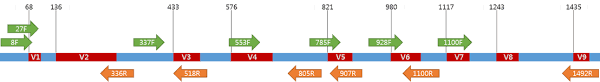
\includegraphics[width=1\linewidth]{images/16S.png}
    \caption{Estructura de las regiones constantes e hipervariables del gen 16S rRNA}
    \label{fig:16S_structure}
\end{figure}
% \begin{figure}[H]
%     \centering
%     \includegraphics[width=1\linewidth]{images/16S_2.png}
%     \caption{Estructura de las regiones variables e hipervariables del gen 16S rRNA}
%     \label{fig:16S_structure2}
% \end{figure}

\hl{hacer denuevo la figura}

El uso de la macromolécula del ARN ribosomal  16S para el estudio de relaciones filogenéticas y de bacterias fue propuesto por Carl Woese a principios de 1970~\cite{olsen1993ribosomal}.
Sus caracteristicas únicas como su presencia en todas las bacterias, su alto grado de conservación (debido a que su función no cambia a través del tiempo) y su tamaño (el cuál permite ser lo suficientemente largo y preciso para la asignación taxónomica, y abordable para análisis bioinformáticos) hacen que hoy en día sea el marcador molecular más utilizado para la identificación de bacterias y comunidades microbianas~\cite{reller2007detection,janda200716s,lopez2023determining,patel200116s}.


Las regiones hipervariables permiten llevar a cabo la caracterización de los microorganismos, siendo la metodología más utilizada el secuenciar parcialmente el gen 16S, es decir, secuenciar una o dos regiones y realizar la asignación taxónomica en base a la región secuenciada. Diversos estudios se han llevado a cabo para determinar los efectos de la selección de la región a utilizar para la identificación, llegandose a determinar que la región hipervariable ha secuenciar influye en los resultados de la comunidad y en la diversidad de microorganismos que se caracteriza~\cite{klindworth2013evaluation,mizrahi2013taxonomic,guo2013taxonomic,soergel2012selection}, y también que ciertas regiones hipervariables permiten identificar mejor ciertos grupos taxonómicos~\cite{buscar}.

%\hl{Evaluation of general 16S ribosomal RNA gene PCR primers for classical and next-generation sequencing-based diversity studies} \hl{The impact of DNA polymerase and number of rounds of amplification in PCR on 16S rRNA gene sequence data, mSphere, vol. 4, 2019}



El gold standard para la identifición de bacterias durante muchos años fue el cultivo convencional en laboratorio, sin embargo, el cultivo puede durar desde días a semanas o incluso meses, y en algunos casos, hay bacterias que no se logran cultivar en laboratorio~\cite{didelot2012transforming}. Es por esto, que las tecnologías de secuenciación de próxima generación se presentaron como una buena alternativa y se empezaron a usar masivamente para secuenciar el gen 16S y caracterizar comunidades al entregar resultados con la suficiente precisión, permitir secuenciar muestras complejas y no solo aislados, y al permitir también secuenciar millones de lecturas al mismo tiempo~\cite{reller2007detection}, haciendo que la forma de caracterizar bacterias sea más estándar y abordable al día de hoy~\cite{woo2008then, tanner1994impact}. 
%El estudio de comunidades microbianas mediante el gen 16S rRNA se ha vuelto una herramienta poderosa tanto en ambientes clínicos como ambientales, permitiendo obtener información de la diversidad de una muestra de manera más rápida y económica que con los métodos tradicionales~\cite{buscar}.
%Las tecnologías de secuenciación  permiten la identificación de bacterias a través de  \hl{signatures/firmas} únicas 

Existen diferentes bases de datos que contienen la información de las secuencias del gen 16S para las diferentes bacterias, como 16S en bases de datos como RDP (Ribosomal Database Project~\cite{cole2014ribosomal}), 16S RefSeq~\cite{}, Greengenes~\cite{desantis2006greengenes}, Silva~\cite{} y el proyecto de microbioma humano (HMP)~\cite{}.
\subsection{Secuenciación de ADN}
Todo ser vivo cuenta con una molécula de ADN que contiene toda la información genética del individuo, esta información se códifica a través de bases nitrogenadas: adenina (A),timina (T), citosina (C) y guanina (G)~\cite{watson1953molecular}. Al día de hoy se han desarrollado diferentes técnicas que permiten determinar la secuencia de nucleótidos en una molecula de ADN, este conjunto de técnicas se conocen como secuenciación de ADN.

Las tecnologías de secuenciación se pueden dividir en tres generaciones, cada una con diferentes características, como los largos de las moleculas a secuenciar, porcentaje de error, costo y cantidad de información que secuencian (throughput). Debido a las diferentes caracterisitcas de cada generación, al analizar las secuencias los análisis bioinformáticos y herramientas a utilizar también cambian~\cite{bierman2014understanding}.

La precisión de estas tecnologías se puede medir mediante la precisión de la lectura raw (precisión al leer un sólo fragmento de ácido nucleico a la vez) o la precisión de los ensamblajes mediante consensos (reconstrucción de genomas completos).

\begin{figure}[H]
    \centering
    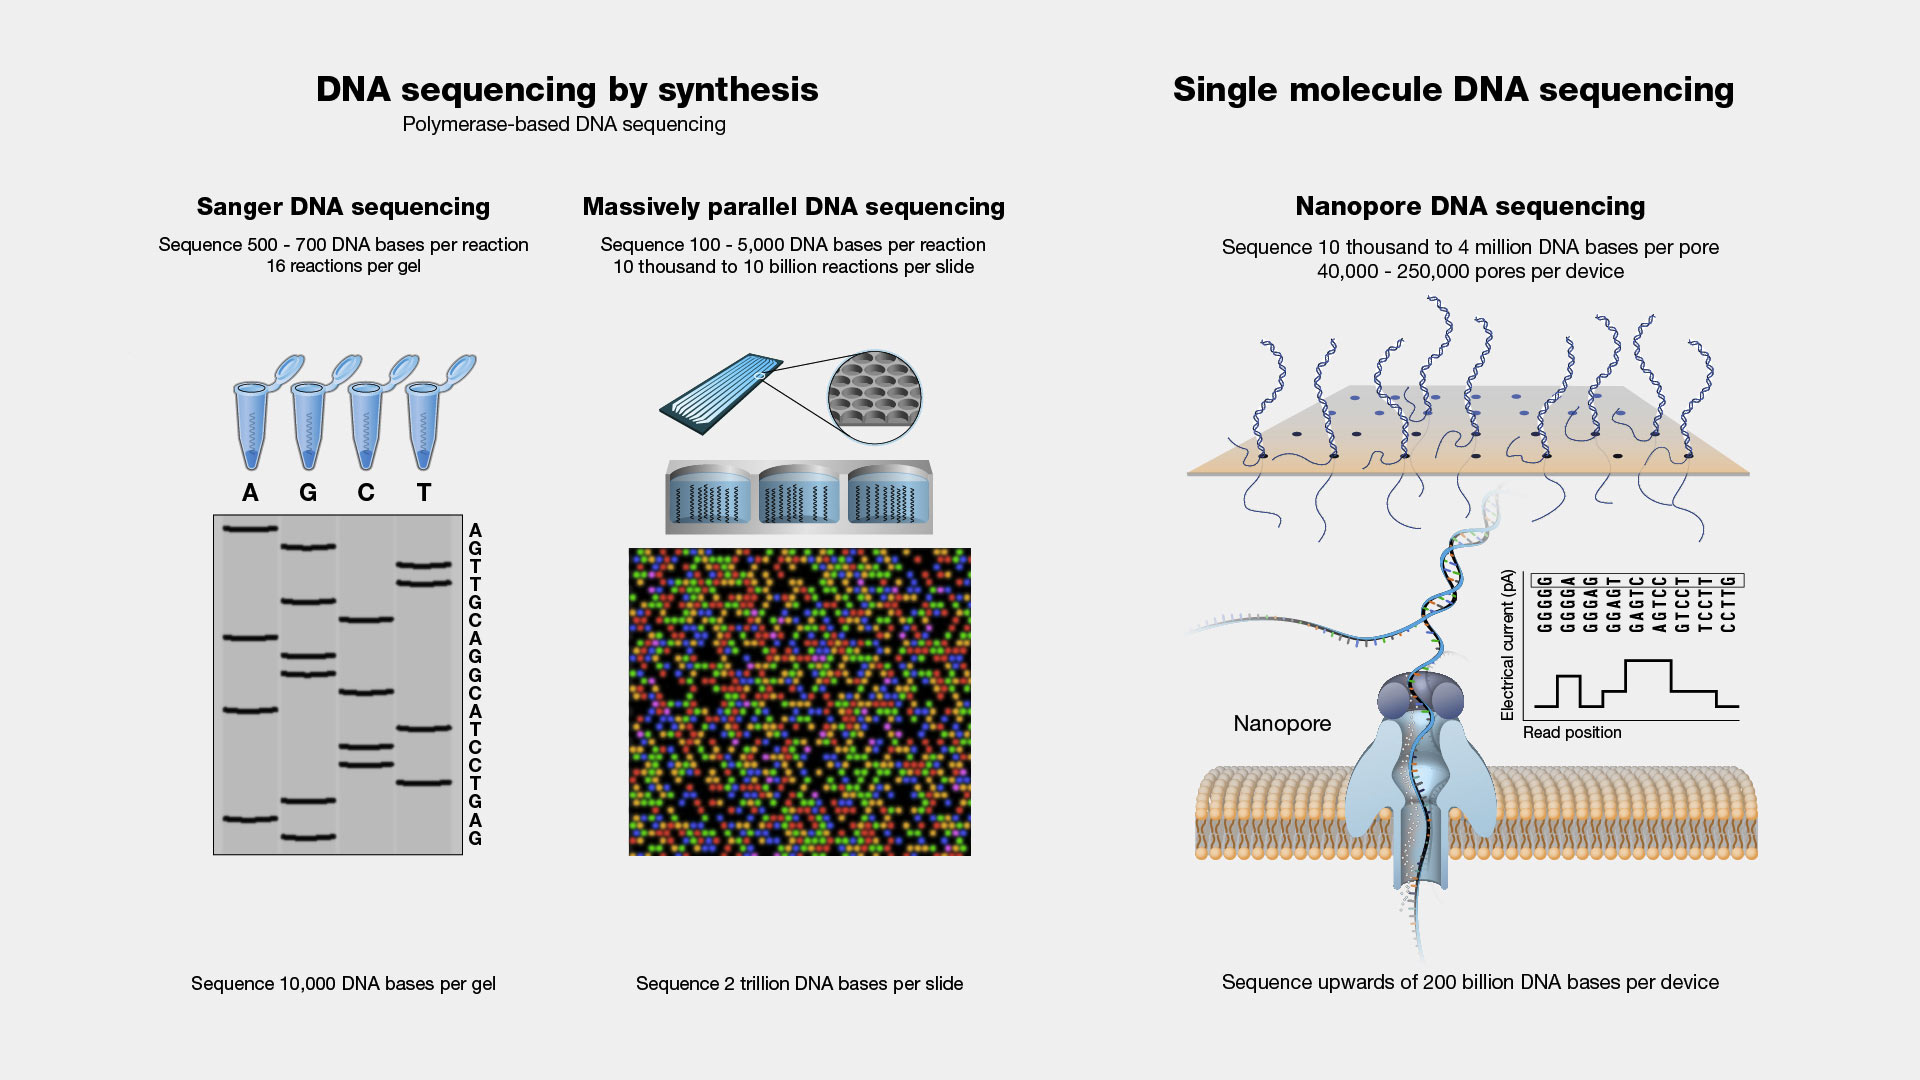
\includegraphics[width=1\linewidth]{images/DNA-Sequencing.jpg}
    \caption{Comparativa tecnologías de secuenciación}
    \label{fig:DNA_sequencing}
\end{figure}

\subsubsection{Primera generación: Sanger}
Frederick Sanger introdujó la primera generación de tecnologías de secuenciación en el año 1977. El método Sanger utiliza el principio de ''terminación de cadena'' para secuenciar material genético~\cite{sanger1975rapid}. 
%Esta técnica replica el ADN utilizan nucleotidos modificados marcados con fluorescencia que detienen el proceso de replicación.
Durante la PCR se añaden nucleótidos modificados (ddNTPs) marcados con fluoroforo que al ser incorporados en la cadena de ADN detienen la elongación de la cadena. Una vez que la reacción ha terminado, se realiza una electroforesis capilar que separa las moleculas de ADN por tamaño y con alta resolución para poder determinar la secuencia de la cadena, generando una única secuencia de como máximo 800 pares de bases por corrida.

La principal ventaja de este método es su alta precisión, siendo ampliamente utilizado en diagnóstico el clínico para la detección de mutaciones puntuales. Además de no requerir capacidad de cómputo ni conocimientos bioinformáticos para la generación de la secuencia.~\cite{BUSCAR}.  
Entre sus principales desventajas se encuentras que es un método laborioso, costoso e ineficiente al trabajar en proyectos de secuenciación de gran escala como por ejemplo genomas completos o metagenómica.
 

\hl{Sanger y el gen 16s}

\subsubsection{Segunda generación: Secuenciación de lecturas cortas}
Las tecnologías de secuenciación de segunda generación como Illumina, IonTorrent, Roche 454 y SOLiD,  utilizaron como base la metodología de interrupción de cadena propuesta por Sanger donde el ADN se fragmenta y cada base se reconoce mediante la emisión de \hl{una señal fluorescente?} al unirse con la hebra complementaria. Con esta generación de secuenciadores se integró el uso de arreglos (que reemplazan la electroforesis capilar), los cuales permiten amplificar el número de copías de cada fragmento de ADN mediante amplificación clonal mediante PCR o un puente PCR \hl{??}, y gracias a esto se logra tener una secuenciación en paralelo de millones de fragmentos cortos de ADN, llegando a una precisión de \hl{99.9}\%, mediante una secuenciación rápida y de bajo costo~\cite{buscar}.


Estas tecnologías de secuenciación utilizan la metodologia denominaada \hl{secuenciación pareada} donde cada fragmento de ADN se secuencia en ambas direcciones, lo que permite obtener fragmentos de hasta \hl{}, siendo el tamaño común para Illumina \hl{}.
Principalmente existen dos metodologías de secuenciación de segunda generación, la secuenciación por síntesis utilizada principalmente por Illumina, y la secuenciación por ligación utilizada por Roche 454 y SOLiD~\cite{mardis2008next}.
La plataforma de secuenciación más utilizada hoy en día es Illumina, la cual en la secuenciación por síntesis luego de fragmentar y añadir los adaptadores, los fragmentos de ADN se unen a la superficie de la celda y se amplifican localmente para formar clusters de cada fragmento de ADN. En cada ciclo de la secuenciación se añaden nucleótidos marcados con fluoróforos, los cuales luego de registrarse se remueven para continuar con el siguiente ciclo. 


Dentro de sus principales ventajas se encuentra su bajo porcentaje de error y costo,y la gran cantidad de herramientas bioinformáticas ya desarrolladas para trabajar con este tipo de datos. Por otro lado, el tamaño de los fragmentos secuenciados es  de su mayor limitante, haciendo más complejos análisis como el ensamblaje de genomas, resolución de regiones repetitivas, etc.



La caracterización de comunidades microbianas con Illumina se ha convertido en el estandar hoy en día, debido a su bajo costo, cantidad de información a secuenciar y alta precisión. Sin embargo las tecnologías de lecturas cortas permiten secuenciar solo una parte del gen 16S rRNA, debido al tamaño de las moleculas que secuencian(lecturas de 200-400pb)~\cite{salipante2014performance}. Esto conlleva a que se deba decidir que región del gen secuenciar, para poder obtener la mayor diversidad posible presente en la muestra, limitando la resolución taxonómica a nivel de género~\cite{buscar} 


%https://sampled.com/short-read-sequencing-vs-long-read-sequencing/#:~:text=Short%2Dread%20sequencing%2C%20as%20the,these%20pieces%20through%20a%20sequencer.
Diversos estudios se han realizado para analizar que región permite obtener esta diversidad de manera precisa~\cite{liu2008accurate,schloss2011reducing}, llegando a descubrirse que ciertos grupos taxonómicos se identifican de mejor manera al utilizar cierta regiones hipervariables~\cite{he2013comparison,claesson2010comparison}.

Al secuenciar el gen 16S con Illumina se sabe que existe presencia de ruido, por lo que se deben realizar filtros como la eliminación de quimeras, eliminación de secuencias singleton y otus raros~\cite{caporaso2011global,auer2017analysis}, realizar denoising con dada~\cite{callahan2016dada2} y unoise~\cite{edgar2016unoise2}. Todas estos filtros y metodologias de trabajo no están disponibles para usarse con TGS como Nanopore y PacBio, debido al porcentaje de error y al tamaño de las lecturas.
Mientras algunos estudios han demostrado, que Nanopore presenta un porcentaje de ruido muy bajo, casi nulo~\cite{szoboszlay2023nanopore}, y a su vez, al secuenciar el gen completo, y no contar con OTUs, o ASV, permite mejorar el rendimiento de los estimadores de riqueza que se basan en estas metodologias, como los índices de chao1~\cite{chao1984nonparametric}, ACE~\cite{chao1992estimating}, o brakaway~\cite{willis2015estimating}


Illumina sobrerepresenta el numero de especies debido al ruido? \hl{Nanopore is preferable over ...}

Es por esto, que las tecnologías de tercera generación como Oxford Nanopore y PacBio se presentan como opciones prometedoras para la secuenciación del gen 16S rRNA, debido a su bajo costo y su capacidad de secuenciar el gen completo en una sola lectura, lo que permite una mayor resolución taxonómica a nivel de especie o incluso de strain~\cite{szoboszlay2023nanopore}~\cite{urban2021freshwater,delahaye2021sequencing}. \hl{revisar estas citas}

\subsubsection{Tercera generación: Secuenciación de lecturas largas}




\subsection{xxx}

El umbral para distinguir especies bacterianas utilizando el gen 16S rRNA es de mínimo 97\% de similitud~\cite{kim2014towards}
\hl{LEEER} https://www.microbiologyresearch.org/content/journal/ijsem/10.1099/ijs.0.059774-0


Las tecnologías de secuenciacin de próxima generación presentan ventajas sobre Sanger a la hora de identificación de patogenos, permitiendo la identificacin en pararelo de bacterias en muestras complejas~\cite{peker2019comparison}, como también presenta ventajas tanto en resolución taxonómica como en precisión~\cite{motro2017next}.

Con la aparición de las tecnologías de secuenciación de segunda y tercera generación~\cite{janda200716s,pollock2018madness}, la secuenciación del gen 16S rRNA se convirtió en es una técnica masiva hoy en día para la caracterización de comunidades microbioanas e identificación tanto de patogenos o aislamiento de bacterias clínicas~\cite{patel200116s}.
Estos métodos requieren la amplificación y secuenciación del gen 16S rRNA y el uso de herramientas biofinformáticas para la identificación y comparación con bases de datos.

\subsubsection{Aplicación tecnologías de secuenciación para la caracterización de comunidades}
Sanger permite la caracterización de bacterias mediante el gen 16S a nivel de especie debido a su alta precisión, sin embargo, permite solo secuenciar muestras aisladas donde solo este presente una bacteria a la vez, por lo que no es útil para la caracterización de comunidades microbianas completas.\hl{muy util en la identidicacion de patogenos clinico}
Con la secuenciación del gen 16S rRNA se obtiene un conjunto de lecturas de ADN, donde cada lectura pertenece a una bacteria presente en la muestra. Estas lecturas se procesan y se comparán con bases de datos existentes para poder realizar la asignación taxonómica y poder identificar la bacteria. Finalmente lo que se obtiene es un perfil de toda la comunidad bacteriana de la muestra, todas las bacterias presentes que las herramientas bioinformáticas pudieron detectar, junto con su abundancia relativa.


\hl{Intrduccion de que es illumina y como funciona illumina}

Ultra-high-throughput microbial community analysis on the Illumina HiSeq and MiSeq platforms.


% \hl{ESTOY VIENDO ACA } https://www.mdpi.com/2076-2607/11/3/804#B1-microorganisms-11-00804
\subsubsection{Oxford Nanopore}
\hl{incluso llegandose a secuenciar en el espacio},
Debido a su capacidad de secuenciar lecturas desde unas pocas kilobases hasta megabases~\cite{amarasinghe2020opportunities}, permite obtener información genómica más completa y contigua que las tecnologías de secuenciación de segunda generación, como Illumina.

Su bajo costo y su portabilidad, que permiten secuenciar 

En sus inicios, la mayor limitante de utilizar Oxford Nanopore era su alto porcentaje de error. En el 2019 estudios reportaban que llegar a una resolución de especie no era aún posible con Nanopore~\cite{winand2019targeting}. Estudios posteriores, determinaron que la precisión de secuenciación se encontraba entre el 92\% al cerca del 96\%~\cite{urban2021freshwater,delahaye2021sequencing}, siendo aún inviable para la asignación taxonómica a nivel de especie \hl{creo que deberia tener cuidado con esto, ya que este paper lo dice, pero otros no}. Sin embargo, con la introducción de la nueva química a finales del 2021, el porcentaje de error reportado por nanopore disminuye notablemente, llegando a un 99.9\% de precisión, permitiendo la resolución taxónomica de especie~\cite{yoon2017introducing}.\hl{buscar más citas}


\section{Herramientas}
El desarrollo de un flujo de trabajo automatizado para la caracterización de comunidades microbionas requiere el uso de diferentes herramientas bioinformáticas para el procesamiento de las secuencias, control de calidad, asignación taxonómica con base de datos, análisis de diversidad, caracterización funcional, etc. Por otro lado, el desarrollo de la aplicación web que estará enlazada al flujo de trabajo, requiere del uso diferentes tecnologías web, librerías y de bases de datos para el almacenamiento de la información, generación de gráficos, y procesamiento de información. A continuación se presentan las principales herramientas a utilizar durante esta tesis.
\subsection{Asignación taxónomica}
La asignación taxónomica en el contexto de secuenciación del gen 16S, es el proceso donde dada una secuencia de ADN, se busca identificar a qué organismo pertenece.
La metodología a utilizar para realizar la asignación va a depender de la tecnología de secuenciación que se haya utilizado,% para Sanger se suele realizar una asignación directa de la lectura que se obtuvo con alguna base de datos como refseq, mientras que para las tecnologías de segunda generación al ser secuencias parciales del gen 16S
para las tencologías de tercera generación lo más común es utilizar la base de datos de RefSeq para buscar la secuencia más parecida en la base de datos mediante alguna herramienta de alineamiento como blast. Algunas metodologias exploran también la corrección de errores de estas secuencias y el clustering de las mismas para mejorar la asignación taxonómica. 
Existen diferentes herramientas para hacer asignación taxonómica de secuencias, algunas incluyen una asignación taxonómica directa a los datos luego del control de calidad, mientras otras herramientas buscan minimizar el error de Oxford Nanopore mediante metodologías de clustering o de algoritmos de maximización de expectativas. 
Algunas de las más utilizadas para trabajar con datos de Oxford Nanopore se presentan a continuación:

\subsubsection{Epi2me}
Plataforma desarrollada por Oxford Nanopore para el análisis de datos secuenciación obtenidos mediante sus dispositivos. 
Integra flujos de trabajo para realizar basecalling y demultiplexación, alineamiento, ensamblaje de SARS-CoV-2, asignación taxonómica de gen 16S, 18S, ITS, y metagenómca, variant calling, entre otros.

Mediante la interfaz gráfica el usuario puede seleccionar el análisis a realizar y configurar los parámetros. Debido a su interfaz de fácil uso permite al usuario abstraerse de la ejecución de herramientas o flujos de trabajo y de la necesidad de contar con recursos computacionales para la ejecución de los mismos.
Los resultados se pueden descargar y visualizar mediante la misma plataforma.
%solo requiere acceso a internet por lo que es una buena alternativa para usuarios que no cuentan con recursos computacionales para el analisis de datos de secuenciacion. Sin embargo, la mayoria de sus flujos de trabajo solo cuenta con análisis primarios y no permite la personalización de los scripts o procesos realizados por lo que en caso de requerir una solución personalizada no se podría llevar a cabo mediante la plataforma. De igual manera, al contar solo con analisis primarios, los analisis posteriores deben ser realizados por el usuario mediante el uso de otras herramientas. 


Para la asignación taxónomica del gen 16S utiliza la herramienta blast con la base de datos de Genbank.

% \begin{itemize}
%     \item Qscore mínimo: 7
%     \item Longitud de lectura mínima: 0
%     \item Longitud de lectura máxima: 0
%     \item e-value máximo: 0.01
%     \item coverage mínimo: 30\%
%     \item Porcentaje de identidad mínimo: 77\%
%     \item max target sequences:
% \end{itemize}
Esta herramienta entrega un archivo en formato CSV con la información de la lectura, asignación taxonómica a nivel de especie, porcentaje de identidad de la asignación, entre otras.
\subsubsection{NanoCLUST}
Nanoclust~\cite{10.1093/bioinformatics/btaa900} es un flujo de trabajo desarrollado en Nextflow para la clasificación de amplicones del gen 16s obtenidos mediante secuenciación de Oxford Nanopore. Incluye pasos previos a la asignación taxonomica, como el basecalling, demultiplexación y control de calidad. Destaca por utilizar un clustering no supervisado (UMAP) y un paso exhaustivo de corrección de lecturas basada en los clusters obtenidos previo a la asignación taxonómica.
Utiliza la base de datos de Genbank para realizar la asignación taxonómica.

Cabe destacar que este flujo de trabajo se encuentra descontinuado ya que fue desarrollado utiilzando Nextflow DSL1 (estándar deprecado en la version 22.10.x). Además, debido a que la herramienta ha dejado de recibir soporte por parte de los desarrolladores, no se han actualizado pasos claves, como el basecalling y demultiplexación (pasos opcionales).

Esta herramienta entrega un archivo csv por cada categoría taxonómica (filo, clase, orden, familia, género, especie) con la cantidad de lecturas asignadas a cada taxonomía. De igual forma, se generan graficos de barra con las asignaciones, y un gráfico de la separación de los clusters. \hl{mejorar}. 
\subsubsection{NanoRTax}

NanoRTax~\cite{RODRIGUEZPEREZ20225350} es un flujo de trabajo desarrollado en Nextflow que cuenta con una interfaz web que permite al usuario visualizar el progreso y resultados del pipeline.
Recibe como entrada los archivos FASTQ, a los cuales se les hace un control de calidad mediante fastp, y a continuación se realiza la asignación taxonómica mediante las herramientas Kraken2, Centrifuge y BLAST. 

Al igual que NanoCLUST, NanoRTax utiliza DSL1 por lo que no es comptabile con versiones nuevas de Nextflow.

El output de esta herramienta \hl{XX}
\subsubsection{EMU}
EMU~\cite{curry2022emu} busca realizar una corrección de errores y mejorar el error de Oxford Nanopore mediante un enfoque basado en algoritmos de maximización de expectativas para generar perfiles taxonómicos de la comunidad microbiona. Permite realizar estos perfiles utilizando diferentes bases de datos, como, la base de datos de Genbank,  RDP y Silva v.138. En el caso de realizar analisis de la región ITS, permite integrar las base de datos de UNITE de fungi y eucariotas.

El output de esta herramienta es un archivo en formato TSV con los perfiles taxonómicos encontrados en cada muestra, es decir, el identificador del taxón, abundancia, especie y la información de todas las categorías taxonómicas. 

\subsubsection{EzBioCloud Microbial Taxonomic Profiling (MTP) pipeline and the PKSSU4.0 database}
En algunos estudios se ha utilizado % https://www.mdpi.com/2076-2607/11/3/804#B1-microorganisms-11-00804 , 
\subsubsection{VSEARCH [35] against the EzBioCloud 16S database.?}

Hoy en día no hay establecidas buenas practicas para el procesamiento del gen 16S rRNA secuenciado mediante Oxford Nanopore, tanto al hablar de la herramienta para hacer asignación taxonómica, como al hablar de la base de datos al utilizar.\hl{leer para ver si citar https://academic.oup.com/femsec/article/97/3/fiab001/6098400}

\subsection{Herramientas bioinformáticas}
Existen diferentes herramientas bioinformáticas que se pueden utilizar para el análisis y manipulación de datos de secuenciación, a continuación se presentan algunas de las más relevantes para este trabajo:

\subsubsection{Guppy}
Guppy es una suite de herramientas provista por Oxford Nanopore para realizar procesamientos de datos de secuenciación básicos. Permite realizar basecalling y demultiplexación, alineamiento, detección de bases modificadas, etc.
\subsubsection{FastQC}
FastQC\cite{andrews2010fastqc} permite visualizar la calidad de los datos mediante métricas estándar de calidad, contenido GC, distribución de tamaños, niveles de duplicación  y contenido de adaptadores.


Genera un reporte en formato html de fácil visualización separado por módulos, donde cada módulo presenta un estado de Aprobado, Fallido o Advertencia (dependiendo de la calidad de los datos). Se desarrollo pensando en tecnología de secuenciación de lecturas cortas, las cuales poseen un porcentaje de error mucho más bajo (menor al 0.1\%) que las tecnologías de secuenciación de tercera generación (entre \hl{xx y xx} \%) y en análisis de genoma completo, por lo que algunos módulos pueden mostrarse como fallidos debido a la naturaleza de los datos de Oxford Nanopore, sin ser datos de baja calidad.
\subsubsection{NanoPlot}
NanoPlot~\cite{10.1093/bioinformatics/btad311} es una herramienta para la evaluación de calidad de datos de secuenciación de lecturas largas, permite visualizar la información de calidad, largo de lecturas y distribución de estas mediantes gráficos interactivos.

Genera un reporte en formato html y gráficos interáctivos que permiten visualizar la calidad de los datos, longitud de las lecturas, distribución de la calidad y longitud, entre otros.
\subsubsection{Fastp}

Fastp\cite{chen2018fastp} es una herramienta de alto rendimiento diseñada para el procesamiento de archivos de secuenciación con calidad (fastq), permite realizar filtrado de secuencias (por calidad, largo), recortar extremos de baja calidad, recortar adaptadores, eliminar colas polyA, etc.
\subsubsection{MultiQC}
MultiQC \cite{ewels2016multiqc} es una herramienta que permite resumir la información obtenida por diferentes herramientas bioinformaticas en un solo informe final. También permite integrar varias muestras en un solo reporte, y multiples pasos de analisis en un solo archivo html.

% Permite una visualización interactiva de los graficos, mediante la cual se puede hacer zoom o quitar muestras de los 

\subsubsection{Seqkit}

\subsubsection{PICRUSt2}
PICRUSt2~\cite{douglas2020picrust2} es una herramienta para la predicción funcional utilizando secuencias marcadoras de genes.
Generalmente se utiliza el gen 16S rRNApara realizar la predicción, pero también se pueden usar otros genes marcadores.

El output entrega archivos en formato CSV con la abundancia de los genes ortologos, la clasificación de las enzimas y las vías metabolicas predichos en cada muestra.

\subsubsection{LEfSe}
LEfSe (Linear discriminant analysis Effect Size)~\cite{segata2011metagenomic}  determina las caracteristicas que permiten explicar las diferencias entre diferentes clases o grupos al combinar pruebas estándar de significancia estadistica junto con pruebas que codifican la consistencia biologica y relevancia del efecto encontrado. 
\subsubsection{vegan package}
Vegan~\cite{dixon2003vegan} es un paquete desarrollado para R que permite realizar análisis de la ecología comunitaria descriptiva. Contiene funciones de análisis de diversidad,  metodos de ordenación comunitaria, análisis de disimilitud, funciones para vegetación y ecologos comunitarios.

% Tiene como objetivo el desarrollo 


\subsubsection{Taxonkit}
Taxonkit~\cite{SHEN2021844} permite la manipulación de información taxónomica de registros de NCBI de una manera eficiente. Dado un identificador taxonómico o un nombre de especie se puede obtener el linage completo de esta.

\subsubsection{csvtk}
csvtk es una herramienta multiplataforma, eficiente y practica para la manipulación de archivos en formato CSV y TSV. Esta herramienta esta desarrollada para utilizarse en conjunto con otras suites de herramientas como TaxonKit, permitiendo obtener resultados de taxonómia de fácil visualización y manipulación para la integración en flujos de trabajo o scripts.
\subsubsection{NCBI database}
Tanto EPI2ME como Nanoclust utilizan la base de datos de ncbi.
\subsection{Lenguajes de programación y Frameworks}
\subsubsection{Nextflow}
Nextflow~\cite{di2017nextflow} es un framework open source para el desarrollo de flujos de trabajo, el cual permite la ejecución de éstos en diferentes entornos computacionales, ya sea en un computador personal, una plataforma de cómputo de alto rendimiento o en la nube. También permite la ejecución de flujos de trabajo de manera paralela, manejando los recursos computacionales de manera eficiente, y sencilla para el usuario.
 Al permitir el desarrollo de flujos de trabajo escalables y reproducibles es una buena alternativa que ha ganado popularidad debido a su facilidad de uso.

Cuenta con una comunidad llamada nf-core que se encarga de desarrollar flujos de trabajo para el análisis de datos biologicos, los cuales son revisados por la comunidad y publicados en su repositorio. Esto permite contar con una gran cantidad de flujos de trabajo disponibles, los cuales pueden ser ejecutados de manera sencilla por los usuarios, pero cabe destacar que hay que tener conocimientos de linea de comando para poder ejecutarlos.


\subsubsection{python?}
\subsubsection{js}

\subsubsection{r?}

\subsubsection{FastAPI}
Framework rápido  y ligero para el desarrollo de APIs modernas de manera ágil utilizando Python y basado en sus anotaciones de tipo estandar.
Utiliza pydantic para la validación de los datos de entrada y salida y starlette para el manejo de las peticiones HTTP. \hl{no estoy 100\% segura}
\subsubsection{SQLalchemy}
Librería de Python que permite la comunicación con base de datos no relacionales de manera sencilla, transformando los registros de la base de datos en objetos utilizables mediante Python. Gestiona la creación de modelos y consultas de forma sencilla.
\subsubsection{Vue.js}
Vue es un framework para la construcción de interfaces de usuario. Se basa en JavaScript, HTML y CSS para proporcionar un modelo de programación declarativo y basado en componentes que permite desarrollar interfaces de manera eficiente.
\subsubsection{TypeScript}  
TypeScript~\cite{bierman2014understanding} es un lenguaje de programación basado en JavaScript, el cual añade sintaxis adicional a JavaScript (o frameworks basados en JS) para soportar la integración de tipado de datos. Al especificar los tipos de datos, TypeScript tiene la capacidad de validarlos e informar errores cuando estos no correspondan.
\subsubsection{Vuetify}
Vuetify es un proyecto de código abierto para la construcción de interfaces utilizando los componentes de Vue. Permite la personalización de los componentes con SASS y SCSS, cuenta con un diseño responsivo, y una gran cantidad de componentes ya predefinidos.
\subsubsection{PostgreSQL}
PostgreSQL es un sistema de gestión de bases de datos relacionales de código abierto que se presentó como la continuación de POSTGRES. Permite el uso de tipos de datos complejos realizar consultas tanto relacionales (SQL) y no relacionales (JSON).

\subsection{Gestores de paquetes}
\subsubsection{Conda}
Conda~\cite{anaconda}  es una herramienta de código abierto, multiplataforma  que permite la gestión de paquetes, dependencias y entornos de desarrollo de manera sencilla. Permite aislar entornos virtuales con caracteristicas especificas, lo que facilita la reproducibilidad de los análisis y la portabilidad de los mismos. \hl{já}
\subsubsection{Apptainer}
Apptainer (antes llamado Singularity~\cite{kurtzer2017singularity}) simplifica la creación y ejecución de contenedores, asegurando el encapsulamiento de los componentes de softwares necesarios para su reproducibilidad y portabilidad.  

\subsection{Métricas para la evaluación de la diversidad microbiana}

Los índices de diversidad permiten evaluar diferentes aspectos de la biodiversidad en una comunidad, como la riqueza, dominancia, y uniformidad de los diferentes individuos en una comunidad. 
Existen diferentes índices de diversidad, los cuales se pueden dividir en índices de riqueza y de \hl{uniformidad/divergencia}, entendiendo la riqueza como el número de especies presentes en una comunidad (sin importar la cantidad de organismos presentes por cada especie) y la uniformidad como la distribución de las abundancias relativas de cada especies.

%Los índices de riqueza permiten evaluar la cantidad de especies presentes en una muestra, mientras que los índices de \hl{uniformidad/divergencia} permiten evaluar la distribución de las especies en la muestra. 
A continuación se presentan algunos de los índices de diversidad más utilizados en la caracterización de comunidades microbianas.   
\subsubsection{Índice de Simpson}
El índice de Simpson mide dominancia y representa la probabilidad de que al seleccionar dos individuos aleatorios de una muestra, ambos pertenezcan a la misma especie. Valores cercanos a 0 indican una alta diversidad y una baja dominancia de algunas especies en especifico

\subsubsection{Índice de Shannon}
El índice de Shannon permite medir la uniformidad de una muestra, Conceptualmente representa el grado de incertidumbre al seleccionar un individuo aleatorio en una comunidad. Este índice suele expresarse mediante su complemento (1-D) donde valores cercanos 0 indican baja diversdiad, es decir alta dominancia de algunas especies en especifico, y valores cercanos a 1 indican alta diversidad, es decir una distribución homogenea entre las especies.

\subsubsection{Índice de Chao1}
